\documentclass[12pt]{jarticle}
\usepackage{TUSIReport}
\usepackage{otf}
\usepackage{ascmac}
\usepackage{listings,jlisting}
\usepackage{url}
\usepackage[dvipdfmx]{graphicx}
\usepackage{here}
\usepackage{subfigure}
\usepackage{amssymb}
\usepackage{multirow}
\usepackage{longtable}
\setlength{\textwidth}{170mm}       % テキストの幅
\setlength{\textheight}{260mm}      % テキストの高さ
\setlength{\oddsidemargin}{-5mm}    % 偶数ページの左マージン
\setlength{\evensidemargin}{0mm}    % 奇数ページの左マージン
\setlength{\topmargin}{-25mm}       % 上のマージン  % 奇数ページの左マージン
\lstset{
  basicstyle={\ttfamily},
  identifierstyle={\small},
  commentstyle={\smallitshape},
  keywordstyle={\small\bfseries},
  ndkeywordstyle={\small},
  stringstyle={\small\ttfamily},
  frame={tb},
  breaklines=true,
  columns=[l]{fullflexible},
  numbers=left,
  xrightmargin=0zw,
  xleftmargin=1zw,
  numberstyle={\scriptsize},
  stepnumber=1,
  numbersep=1zw,
  lineskip=-0.5ex
}
\begin{document}
%%%%%%%%%%%%%%%%%%%%%%%%%%%%%%%%%%%%%%%%%%%%%%%%%%%%%%%%%%%%%%
% 表紙を出力する場合は,\提出者と\共同実験者をいれる
% \提出者{科目名}{課題名}{提出年}{提出月}{提出日}{学籍番号}{氏名}
% \共同実験者{一人目}{二人目}{..}{..}{..}{..}{..}{八人目}
%%%%%%%%%%%%%%%%%%%%%%%%%%%%%%%%%%%%%%%%%%%%%%%%%%%%%%%%%%%%%%
\提出者{情報工学実験2}{実験テーマ5 教育システム設計}{2020}{9}{28}{4619023}{加藤零}
\共同実験者{}{}{}{}{}{}{}{}

%%%%%%%%%%%%%%%%%%%%%%%%%%%%%%%%%%%%%%%%%%%%%%%%%%%%%%%%%%%%%%
% 表紙を出力しない場合は,以下の「\表紙出力」をコメントアウトする
%%%%%%%%%%%%%%%%%%%%%%%%%%%%%%%%%%%%%%%%%%%%%%%%%%%%%%%%%%%%%%
\表紙出力

%%%%%%%%%%%%%%%%%%%%%%%%%%%%%%%%%%%%%%%%%%%%%%%%%%%%%%%%%%%%%%
% 以下はレポート本体である.別途 TeXファイルを作成し \input 使っても良い
%%%%%%%%%%%%%%%%%%%%%%%%%%%%%%%%%%%%%%%%%%%%%%%%%%%%%%%%%%%%%%

\section{要旨}
高校で学習したベイズの定理が最尤推定を行う際にどのように応用されるかを学習・検討する.今回はある問いに関する能力推定を題材とする.

\section{目的}
統計モデルを用いた分析は,商品の推薦や迷惑メールの削除機能など,身近な機能を支える基本的な技術となっている.本実験では,このような統計モデルを用いた分析に欠かせない,パラメタの推定の方法について基本的な技術を習得することを目的とする.

\section{理論}
\subsection{項目反応理論基礎}
項目反応理論では,ある受験者$j$がある項目$i$に正答する$x_i,j=1$確率を以下の式でモデル化する.
\begin{equation}
    P(x_{i,j}=1 \mid \theta _j,a_i,b_i)= P_i(x_{i,j}=1 \mid \theta _j)=P_i(\theta _j)=\frac{1}{1+\exp\{-Da_i(\theta_j -b_i)\}}
\end{equation}
ここで$\theta_j$は受検者の能力パラメタ,$a_i$は項目の識別力パラメタ,$b_i$は項目の困難度パラメタである.また,$D=1.7$としたとき,このモデルは以下の特徴がある.
\begin{enumerate}
    \item $\theta_j=b_i$の場合正答確率は50\%となる.
    \item $\theta_j=b_i$での正答率の傾きは$a_i$に比例する,
    \item $a_i=1,b_i=0$のとき,この関数は累積標準正規分布の良い近似となる.
\end{enumerate}
識別パラメータが0に近い項目は,能力値によらず一定の正答率となるような,能力に関係ない項目となる.また,困難度パラメタが大きな項目では正答に必要な能力値が大きくなる,
\subsection{最尤推定を用いた受検者能力の推定}
項目反応理論を用いた受検者の能力値の推定も最尤推定と同様に計算する.例えば,今ある問題に正答した$(x_{i,j})$とする.この時の受検者の能力値は以下の数式を考えれば良い.
\begin{equation}
    \hat{\theta} = \mathop{\rm arg~max}\limits_{\theta} P(\theta \mid x_{i,j}=1)
\end{equation}
ただし,$P(\theta_j \mid x_{i,j}=1)$はのIRTモデルに従って直接は与えられていないため,ベイズの定理より,$P(x_{i,j}=1 \mid \theta_j)$を用いて考える.
\begin{eqnarray}
    P(\theta \mid x_{i,j}=1)=\frac{P(\theta_j)}{P(x_{i,j}=1)}P_i(x_{i,j}=1 \mid \theta_j)
\end{eqnarray}
ここで,$P(x_{i,j})$はその問題に正答できる確率であるが,変数$\theta_j$と独立な変数であるため,$\mathop{\rm arg~max}\limits_{\theta}$を考える上で定数とみなすことができる.従って,以下の式を考えても結果は変わらない.
\begin{eqnarray}
    \hat{\theta} &=& \mathop{\rm arg~max}\limits_{\theta} P(\theta \mid x_{i,j}=1) \\
    &=& \mathop{\rm arg~max}\limits_{\theta}P(\theta) P(x_{i,j}=1\mid\theta)
\end{eqnarray}
$P(\theta)$は能力値が一般にどのような分布をしているかを表すので,標準正規分布していると仮定できる.
\begin{eqnarray}
    P(\theta)=\frac{1}{\sqrt{2\pi}}\exp \left(-\frac{\theta ^2}{2}\right)
\end{eqnarray}
また,誤答した場合も同様に以下のように考えることができる.
\begin{eqnarray}
    \hat{\theta} &=& \mathop{\rm arg~max}\limits_{\theta} P(\theta \mid x_{i,j}=0)\\
    &=& \mathop{\rm arg~max}\limits_{\theta}P(\theta) P(x_{i,j}=0\mid\theta_j)\\
    &=& \mathop{\rm arg~max}\limits_{\theta}P(\theta)(1- P(x_{i,j}=1\mid\theta_j))
\end{eqnarray}
このような関数を考えることで,ある問題に正答,あるいは誤答した場合の受験者の能力値を推定することが可能である.また,$P(\theta)$は問題に正答したという事実を受け取る前の確率であり,事前確率と呼ばれることがある.加えて,$P(\theta \mid x_{i,j})$は問題に正答あるいは誤答したという事実を受け取ったあとの確率なので,事後確率と呼ばれることがある.また,項目反応理論では,項目情報量関数と呼ばれる指標が非常に重要となる.項目情報量関数とは,項目反応関数について項目への反応から能力値を推定する際のフィッシャー情報量を算出したものであり,2パラメタロジスティックモデルでは以下のような式となる.
\begin{eqnarray}
    I_i(\theta)=D^2a_i^2 P_i(\theta)(1-P_i(\theta))
\end{eqnarray}
フィッシャー情報量は一般に
$\hat{\theta}$
の標準誤差
${\rm se}(\hat{\theta})$
と以下の関係を持つ
\begin{eqnarray}
    {\rm se}(\hat{\theta})=I_i(\hat{\theta})^{-\frac{1}{2}}=\frac{1}{\sqrt{I_i(\hat{\theta})}}
\end{eqnarray}
そのため,この項目情報量を用いることで,推定された$\hat{\theta}$に対してどの程度標準誤差があるかを見積もることができる.
\section{課題}
\subsection{課題2-1}
\begin{shadebox}
    \quad 課題1-3で解いた項目について,項目反応関数の概形を描け.
\end{shadebox}
\vspace{\baselineskip}
特性パラメタは表1のようになる.そしてこれらのパラメタを用いると項目反応関数の概形は図1のようになる.
\begin{table}[h]
    \centering
    \caption{各問題の特性パラメタ}
    \begin{tabular}{|c|r|r|} \hline
        問題 & \multicolumn{1}{|c|}{aパラメタ} & \multicolumn{1}{|c|}{bパラメタ} \\
        \hline\hline
        1    & 0.39117                         & -0.74843                        \\ \hline
        4    & 0.32597                         & 0.03162                         \\ \hline
        7    & 0.6118                          & -0.48178                        \\ \hline
        10   & 0.33723                         & -0.63348                        \\ \hline
        13   & 0.67552                         & -0.57458                        \\ \hline
        16   & 0.89931                         & -1.14805                        \\ \hline
        19   & 0.64296                         & 0.20626                         \\ \hline
        22   & 0.47439                         & -0.1113                         \\ \hline
        25   & 0.34592                         & -1.07541                        \\ \hline
        28   & 0.63141                         & -1.70127                        \\ \hline
    \end{tabular}
\end{table}
\begin{figure}[h]
    \begin{center}
        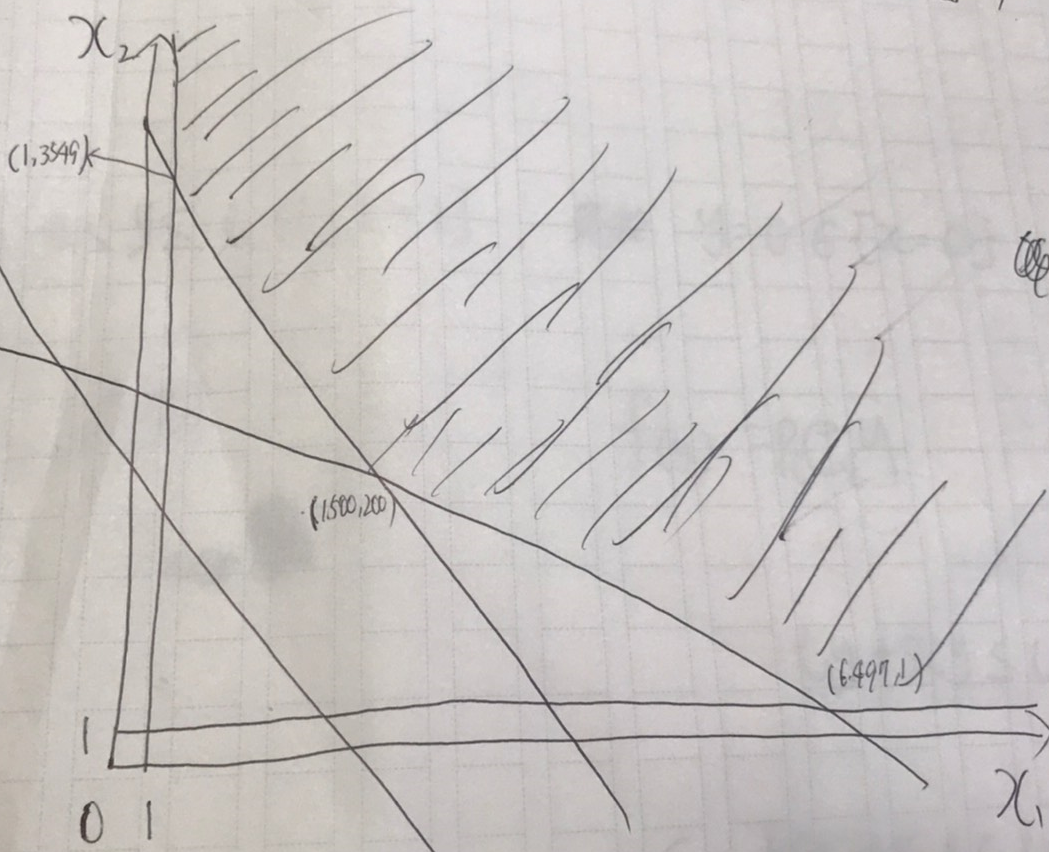
\includegraphics[bb=0 0 889 434,height=8cm]{1.png}
    \end{center}
    \caption{項目反応関数の概形}
    \label{fig1}
\end{figure}
\subsection{課題2-2}
\begin{shadebox}
    \quad 課題2-1で描いたグラフを参考に,それらの項目がどのような項目であったのか考察せよ.
\end{shadebox}
\vspace{\baselineskip}
図1のグラフにおいてそれぞれの項目の傾きに着目すると,大きく分けて二つのグループに分けることができる.まず,傾きの変化が激しいものはitem7,13,16,19,28である.傾きの変化が激しいということから,能力値に依存した項目であり,高い正答率を取得するために必要な能力値も高くなっている,また,正答率50\%となる場合,グラフにおいて右からitem19,7,13,16,28となっており,正答率50\%を達成する際にはこれらの順に難しいと考えられる.一方のitem1,4,0,22,25は傾きに変化がすくないことから,能力値に関係なく比較的正答率が高い問題であったといえる.正答率50\%となる場合,グラフにおいて右からitem4,22,10,1,25となっており,正答率50\%を達成する際にはこれらの順に難しいと考えられる.以上から傾きの変化が少ない問題は正答率をあげる場合に能力値を必要としないため比較的簡単な問題と推測することができ,一方で傾きの変化が激しい問題は正答率を上げる場合に能力値を必要とするため難しい問題であると推測できる.また,同系統の概形のグラフでは右にあるほど難しいと考えられる.
\subsection{課題2-3}
\begin{shadebox}
    \quad $\theta_j=b_i$の場合,正答確率は50\%になることを証明せよ.
\end{shadebox}
\vspace{\baselineskip}
$\theta_j=b_i$を式1に代入すれば良い.
\begin{eqnarray*}
    P(\theta_j)&=&\frac{1}{1+\exp\{-Da_i(\theta_j -b_i)\}}\\
    &=&\frac{1}{1+\exp\{-Da_i(b_i -b_i)\}}\\
    &=&\frac{1}{1+\exp(0)}\\
    &=&0.5
\end{eqnarray*}
よって50\%となる.

\subsection{課題2c-1}
\begin{shadebox}
    \quad $\theta_j=b_i$での項目反応関数の傾きは$a_i$に比例することを証明せよ.
\end{shadebox}
\vspace{\baselineskip}
式1を$\theta_j$で微分した後に$\theta_j=b_i$を代入すれば良い.
\begin{eqnarray*}
    \frac{d}{d \theta_j}P(\theta_j)&=&\frac{Da_i\exp\{-Da_i(\theta_j -b_i)\}}{<1+\exp\{-Da_i(\theta_j -b_i)\}>^2}\\
    &=&\frac{Da_i\exp(0)}{(1+\exp(0))^2}\\
    &=&\frac{1}{4}Da_i
\end{eqnarray*}
この式は$a_i$に関して比例するため題は示された.
\subsection{課題2–4}
\begin{shadebox}
    \quad 課題1-3で解いた項目から1題選びその正誤から描かれる事後分布のグラフを示せ.
\end{shadebox}
\vspace{\baselineskip}
ここではitem19を例として考える.すると正答確率および誤答確率のグラフは図2のようになる.また,正答および誤答の事後分布はこれらに正規分布を掛け合わせたものであるため,図3のようになる.
\clearpage
\begin{figure}[h]
    \begin{center}
        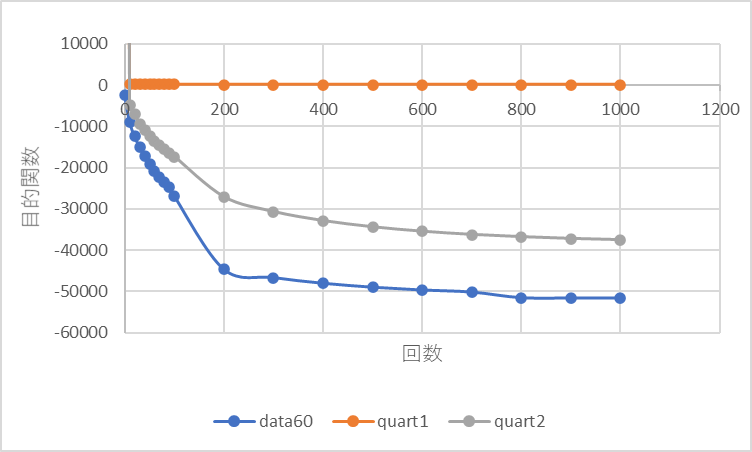
\includegraphics[bb=0 0 407 239,height=8cm]{2.png}
    \end{center}
    \caption{item19の正答確率と誤答確率}
    \label{fig2}
\end{figure}
\begin{figure}[h]
    \begin{center}
        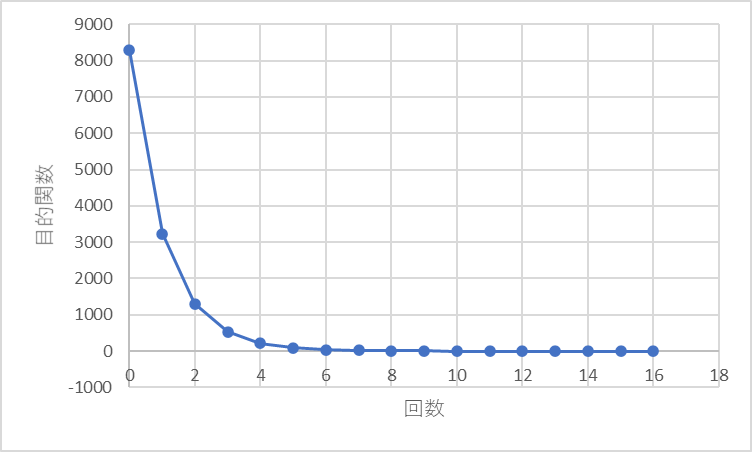
\includegraphics[bb=0 0 393 232,height=8cm]{3.png}
    \end{center}
    \caption{item19の正答事後確率と誤答事後確率}
    \label{fig3}
\end{figure}
\subsection{課題2–5}
\begin{shadebox}
    \quad 課題2-4で描いた事後分布から能力値を推定せよ.またその時の標準誤差を求めよ.
\end{shadebox}
\vspace{\baselineskip}
item19に関して正答しているため式4,5を利用して$\hat{\theta}$を求めることは,図3の正答事後分布が最大となる際の$\theta$を求めることと同等であるから0.5となる.標準誤差は式10,11より求めることができる.
\begin{eqnarray*}
    I_i(\theta)=I_i(0.2)
    &=&1.7^2 0.64296^2P_i(0.5)(1-P_i(0,5))\\
    &\simeq&0.29111
\end{eqnarray*}
これを式11に代入すると,
\begin{eqnarray*}
    {\rm se}(\hat{\theta})=I_i(\hat{\theta})^{-\frac{1}{2}}=\frac{1}{\sqrt{0.29111}}\simeq1.85340
\end{eqnarray*}
となる.よって標準誤差は約1.85340となる.
\subsection{課題2–6}
\begin{shadebox}
    \quad $\theta$の刻み幅を0.1以外に2パターンを自ら適当に変更した場合の能力値と標準誤差の結果を記述し,結果について考察せよ.
\end{shadebox}
\vspace{\baselineskip}
$\theta$の刻み幅を0.4と0.8にした場合について考察する.$\theta$の刻み幅を0.4としたときの正答確率および誤答確率のグラフは図4のようになる.また,正答および誤答の事後分布はこれらに標準正規分布を掛け合わせたものであるため,図5のようになる.同様にして$\theta$の刻み幅を0.8とすると,図6,7のようになる.
\begin{figure}[h]
    \begin{center}
        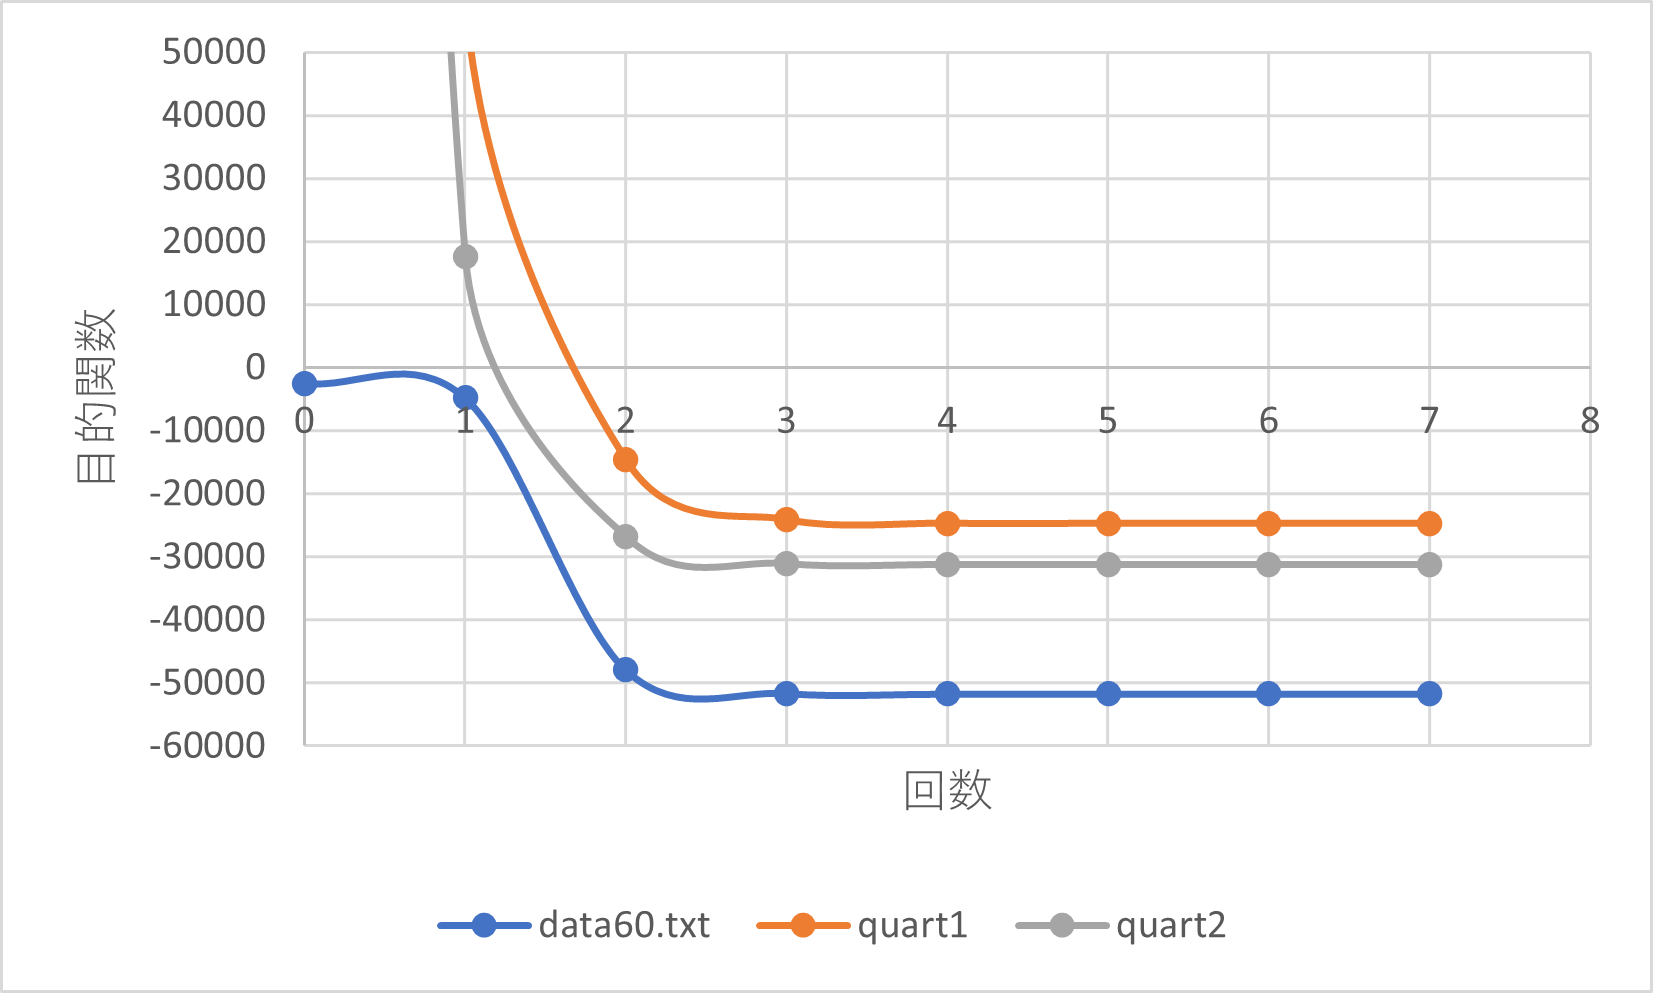
\includegraphics[bb=0 0 412 245,height=8cm]{4.png}
    \end{center}
    \caption{item19の正答確率と誤答確率(刻み幅=0.4)}
    \label{fig4}
\end{figure}
\clearpage
\begin{figure}[h]
    \begin{center}
        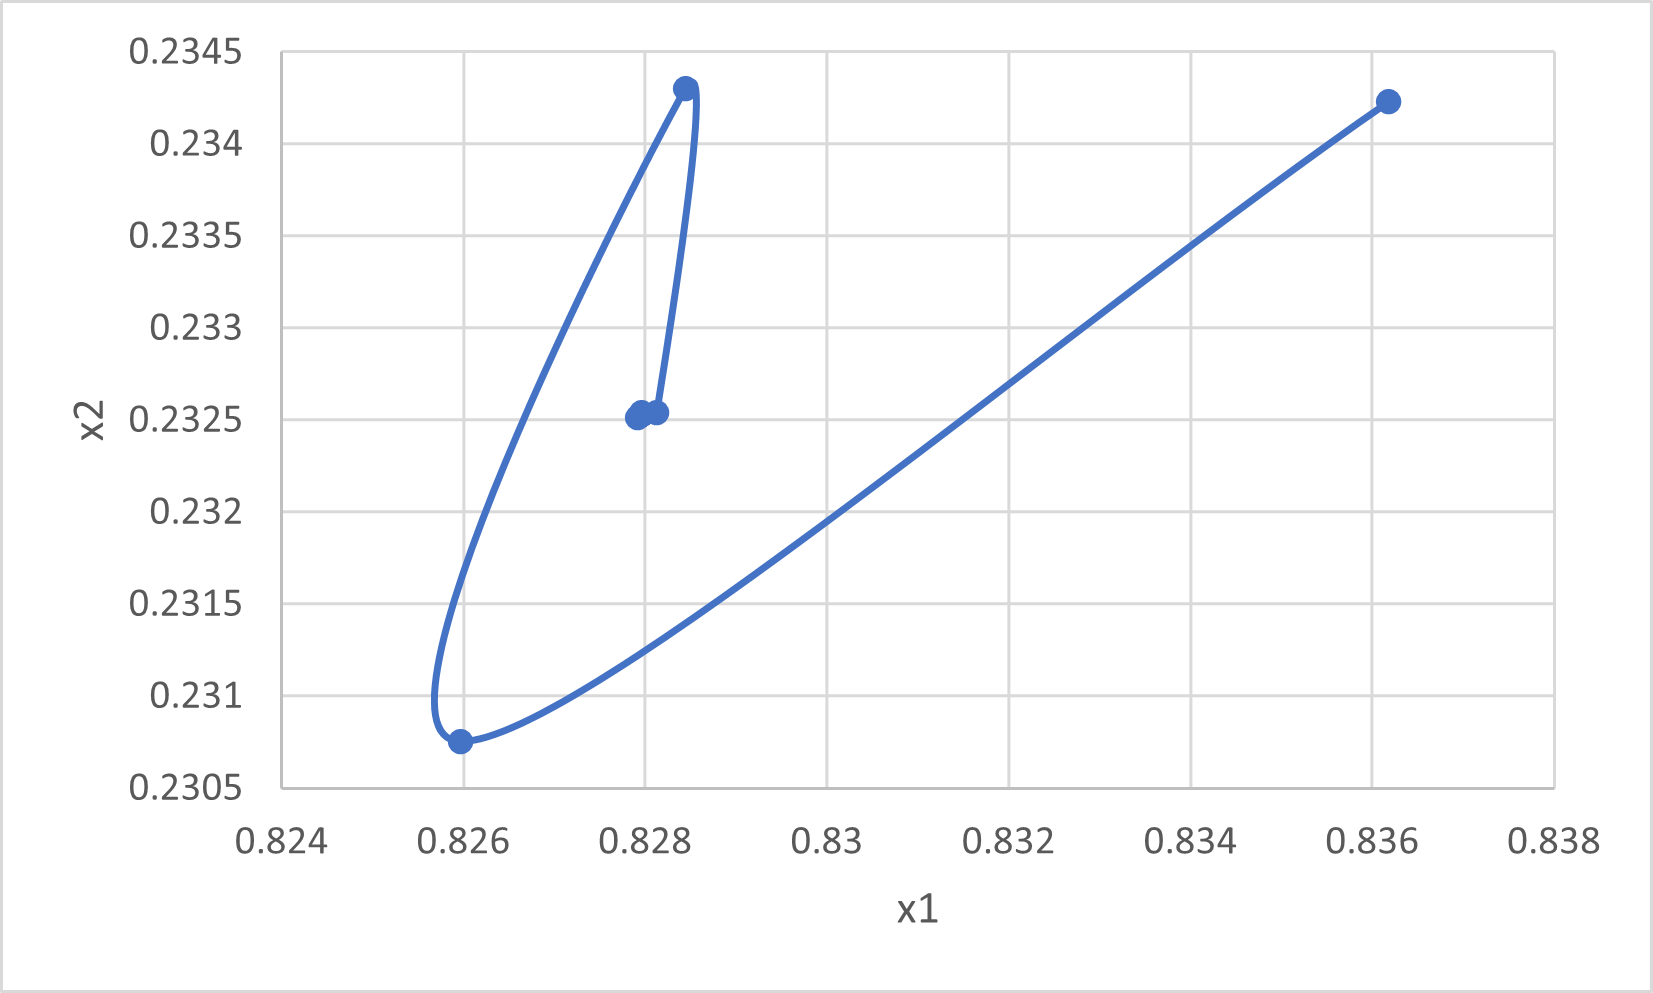
\includegraphics[bb=0 0 412 245,height=8cm]{5.png}
    \end{center}
    \caption{item19の正答事後確率と誤答事後確率(刻み幅=0.4)}
    \label{fig5}
\end{figure}
\begin{figure}[h]
    \begin{center}
        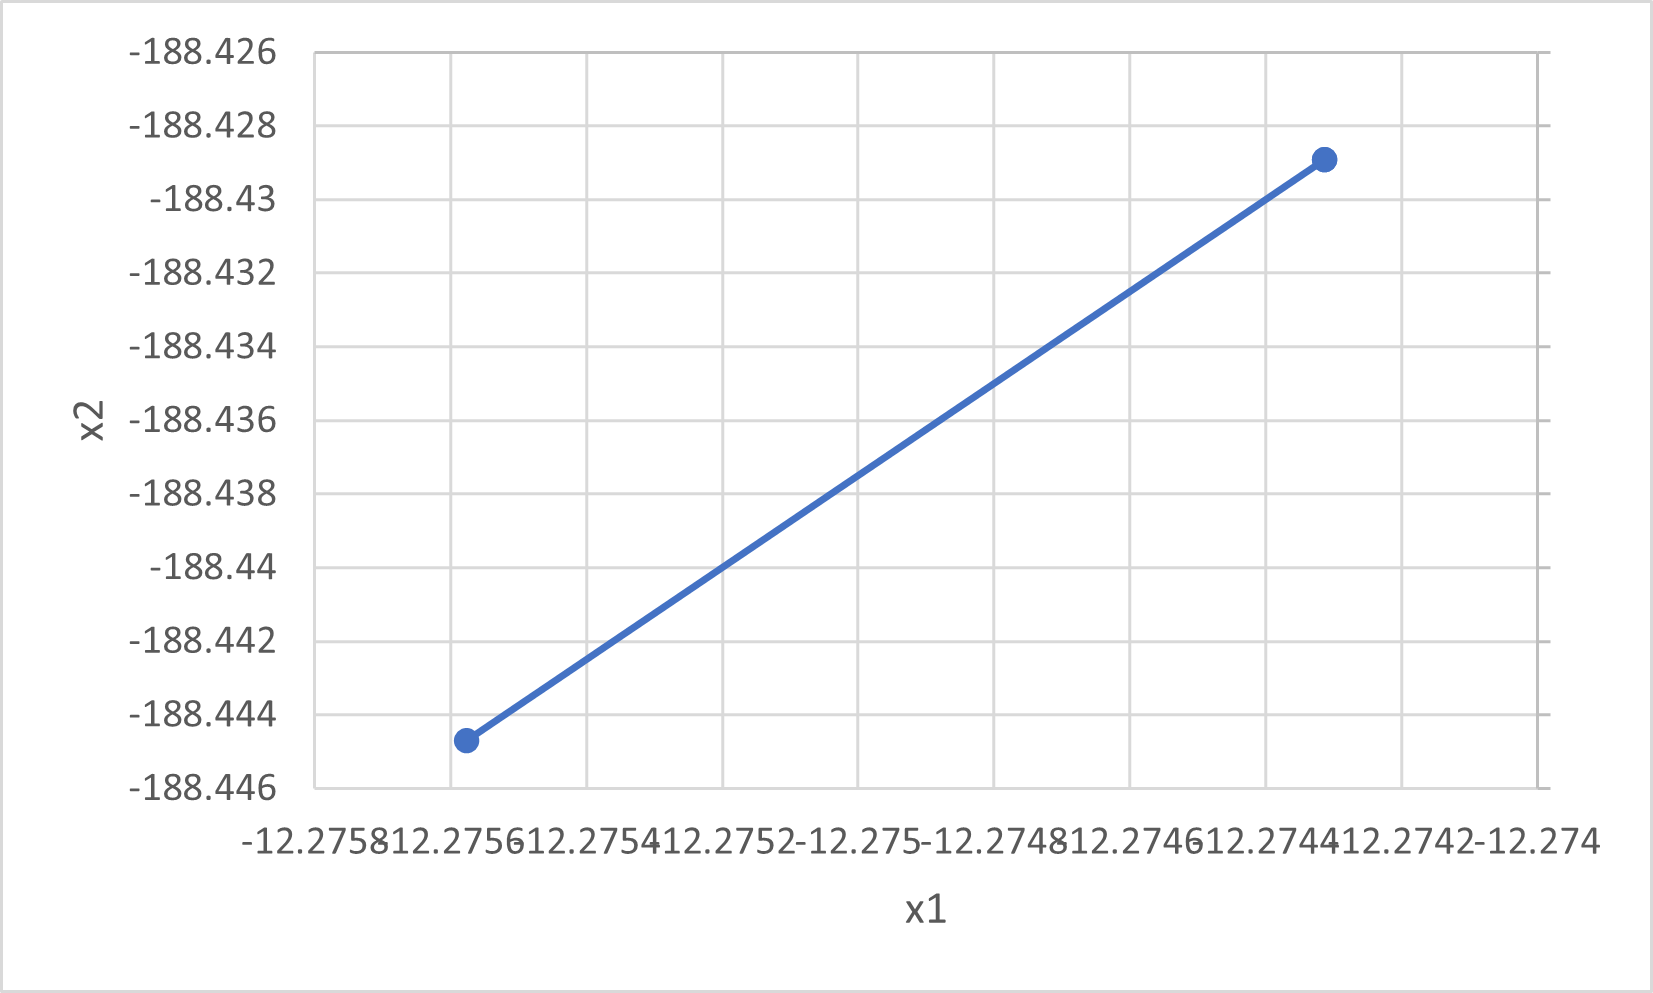
\includegraphics[bb=0 0 412 245,height=8cm]{6.png}
    \end{center}
    \caption{item19の正答確率と誤答確率(刻み幅=0.8)}
    \label{fig6}
\end{figure}
\clearpage
\begin{figure}[h]
    \begin{center}
        \includegraphics[bb=0 0 412 245,height=8cm]{7.png}
    \end{center}
    \caption{item19の正答事後確率と誤答事後確率(刻み幅=0.8)}
    \label{fig7}
\end{figure}

図5,7から能力値を導出すると$\theta$の刻み幅が0.4の場合に0.4, 0.8の場合は0.8となり標準誤差はそれぞれ,1.84003と1.92695となった,このことから,刻み幅を変化させると推定される能力値が変化してしまうといえる.また,刻み幅が広がり,式5を成立させる$\theta$が幅から外れてしまうと,$\theta$は小さくなったり大きくなったりしてしまい,これにより標準誤差が変化しているといえる.このように最尤推定により求まる値は刻み幅を変化させると推定値も変化してしまうため正しい値と断言できない. より真値に近しいものを求める際には刻み幅を変化させてその変異を確認するのが有効だと推測できる.

\subsection{課題2–6}
\begin{shadebox}
    \quad 能力値の事前分布が平均0.5,分散1の正規分布に従うと仮定された場合,自分の能力値と情報量について計算し,結果について考察せよ.
\end{shadebox}
\vspace{\baselineskip}
今回の題の条件に従った場合も分散は標準正規分布と同じである,つまり,式6が
\begin{eqnarray}
    P(\theta)=\frac{1}{\sqrt{2\pi}}\exp \left(-\frac{(\theta-0.5) ^2}{2}\right)
\end{eqnarray}
のように変化する.この式のグラフは標準正規分布のグラフを右に0.5移動したものである.故に受験者の能力の分布が標準正規分布と比べて向上したものである.先ほどと同様の手段で能力値を推定してみる.正答確率および誤答確率のグラフは図8のようになる.また,正答および誤答の事後分布はこれらに正規分布を掛け合わせたものであるため,図9のようになる,図9より能力値は0.9と推定することができる.
\begin{eqnarray*}
    I_i(\theta)=I_i(0.9)
    &=&1.7^2 0.64296^2P_i(0.5)(1-P_i(0,5))\\
    &\simeq&0.25955
\end{eqnarray*}
これを式11に代入すると,
\begin{eqnarray*}
    {\rm se}(\hat{\theta})=I_i(\hat{\theta})^{-\frac{1}{2}}=\frac{1}{\sqrt{0.25955}}\simeq1.96287
\end{eqnarray*}
となり,標準誤差は約1.96287だとわかる.
\begin{figure}[h]
    \begin{center}
        \includegraphics[bb=0 0 506 291,height=8cm]{8.png}
    \end{center}
    \caption{item19の正答確率と誤答確率(能力値が平均0.5,分散1の正規分布に従うと仮定)}
    \label{fig8}
\end{figure}
\begin{figure}[h]
    \begin{center}
        \includegraphics[bb=0 0 506 291,height=8cm]{9.png}
    \end{center}
    \caption{item19の正答事後確率と誤答事後確率(能力値が平均0.5,分散1の正規分布に従うと仮定)}
    \label{fig9}
\end{figure}

今回の題において標準正規分布を右に0.5移動させた分布に従っているという仮定により,推定した能力値が0.5から0.9に向上したといえる.また,正答確率の関数は変化していないことと標準正規分布を右に0.5移動させた分布に従っているということにより,正答確率事後分布は山が全体的に右によっており高さも高くなっている。一方で誤答確率事後分布は左によって山の高さも低くなっている.これはある問題に関して正答する確率と誤答する確率は互いに依存しているということが原因で引き起こされた現象である.そして,これらを原因としてフィッシャー情報量や標準誤差に変化が生まれている.
\section{まとめ}
今回の演習・課題により項目反応理論を用いることである受験者が正答または誤答する確率を数式によってモデル化することができるということがわかった.また,能力値の分布を仮定することで受験者の能力値を推定することができるが,それは必ずしも真値に近いといえない.


% 参考文献
\begin{thebibliography}{99}
    \label{sannkoubunnkenn_chapter}
    \bibitem{} 高校数学の美しい物語\\
    \url{https://mathtrain.jp/gaussdistribution}\\
    最終閲覧日; 2020/10/5
    \bibitem{} 項目反応理論(Item Response Theory:IRT)に関連する用語説明 Ver1.1\\
    \url{http://www.med.oita-u.ac.jp/mededuc/cbt/riron_yougo.pdf}\\
    最終閲覧日; 2020/10/5
\end{thebibliography}

%%%%%%%%%%%%%%%%%%%%%%%%%%%%%%%%%%%%%%%%%%%%%%%%%%%%%%%%%%%%%%
\end{document}